\section{The Decision Model}
\label{sec:decision_model}

The complexity of large-scale maintenance scheduling extends beyond the combinatorial explosion of the search space, it fundamentally involves the reconciliation of conflicting objectives. While traditional optimization approaches often collapse these dimensions into a linear weighted sum of generic ``Risk'' and ``Cost'' indicators, real-world decision-making requires a granular assessment of strategic goals. To address this, a decision matrix $\mathbf{X} \in \mathbb{R}^{N \times M}$ is constructed by transforming raw operational data into $M=7$ criteria. These are designed to capture specific concerns of the grid operator, categorized into three blocks: Safety, Robustness, and Strategy. Table~\ref{tab:notation} in \ref{app:notation} summarizes the notation used throughout this section.

\subsection{Spatial and Temporal Reconstruction}

A major challenge in analyzing anonymized grid data is the absence of explicit geographical coordinates, which hinders the assessment of location-dependent criteria such as environmental impact on National Parks or economic risks near ski resorts.

To overcome this, the analysis relies on the assumption that interventions located in close geographic proximity share common stressors, leading to correlated variations in their risk profiles over time. Similarity between interventions $i$ and $j$ is measured by the sign concordance of their temporal variations $\Delta \bar{r}_{i,t} = \bar{r}_{i,t+1} - \bar{r}_{i,t}$:
\[
\sigma_{ij} = \sum_{t=1}^{T-1} s(\Delta \bar{r}_{i,t}, \Delta \bar{r}_{j,t}), \quad
s(a,b) = \begin{cases}
+1 & \text{if } \text{sgn}(a) = \text{sgn}(b) \\
-1 & \text{if } \text{sgn}(a) = -\text{sgn}(b) \neq 0 \\
0 & \text{otherwise}
\end{cases}
\]
The resulting matrix is normalized by $\hat{\sigma}_{ij} = \sigma_{ij} / \sqrt{\sigma_{ii} \cdot \sigma_{jj}}$. Correlations are then transformed into dissimilarities via the linear mapping $d_{ij} = (1 - \hat{\sigma}_{ij}) / 2$. 

Since positive correlation indicates proximity but negative correlation does not imply distance, only positive correlations are used in the Multidimensional Scaling (MDS) embedding. Non-Metric MDS via the SMACOF algorithm \cite{smacof} is applied to project the interventions into a 2D Euclidean space $\mathbb{R}^2$. The resulting point cloud is affinely scaled to fit the bounding box of France. While this reconstruction is an approximation, it enables computing the fuzzy proximity of an intervention $i$ to specific sensitive zones $Z$, allowing for the evaluation of spatially-aware criteria:
\[
\mu_{Z}(i) = \begin{cases}
1 & \text{if } d(i, Z) \le d_{min} \\
\frac{d_{max} - d(i, Z)}{d_{max} - d_{min}} & \text{if } d_{min} < d(i, Z) < d_{max} \\
0 & \text{if } d(i, Z) \ge d_{max}
\end{cases}
\]
For ski areas, $d_{min} = 30$ km and $d_{max} = 80$ km, capturing the broader regional influence of winter tourism infrastructure. For regional natural parks, $d_{min} = 1$ km and $d_{max} = 10$ km, reflecting that environmental sensitivity is primarily determined by whether an intervention occurs within or immediately adjacent to the protected area.

Figure~\ref{fig:interventions_map} illustrates the resulting spatial reconstruction, showing the distribution of interventions alongside the sensitive zones (regional natural parks and ski areas) used to compute the fuzzy memberships.

\begin{figure}[ht]
    \centering
    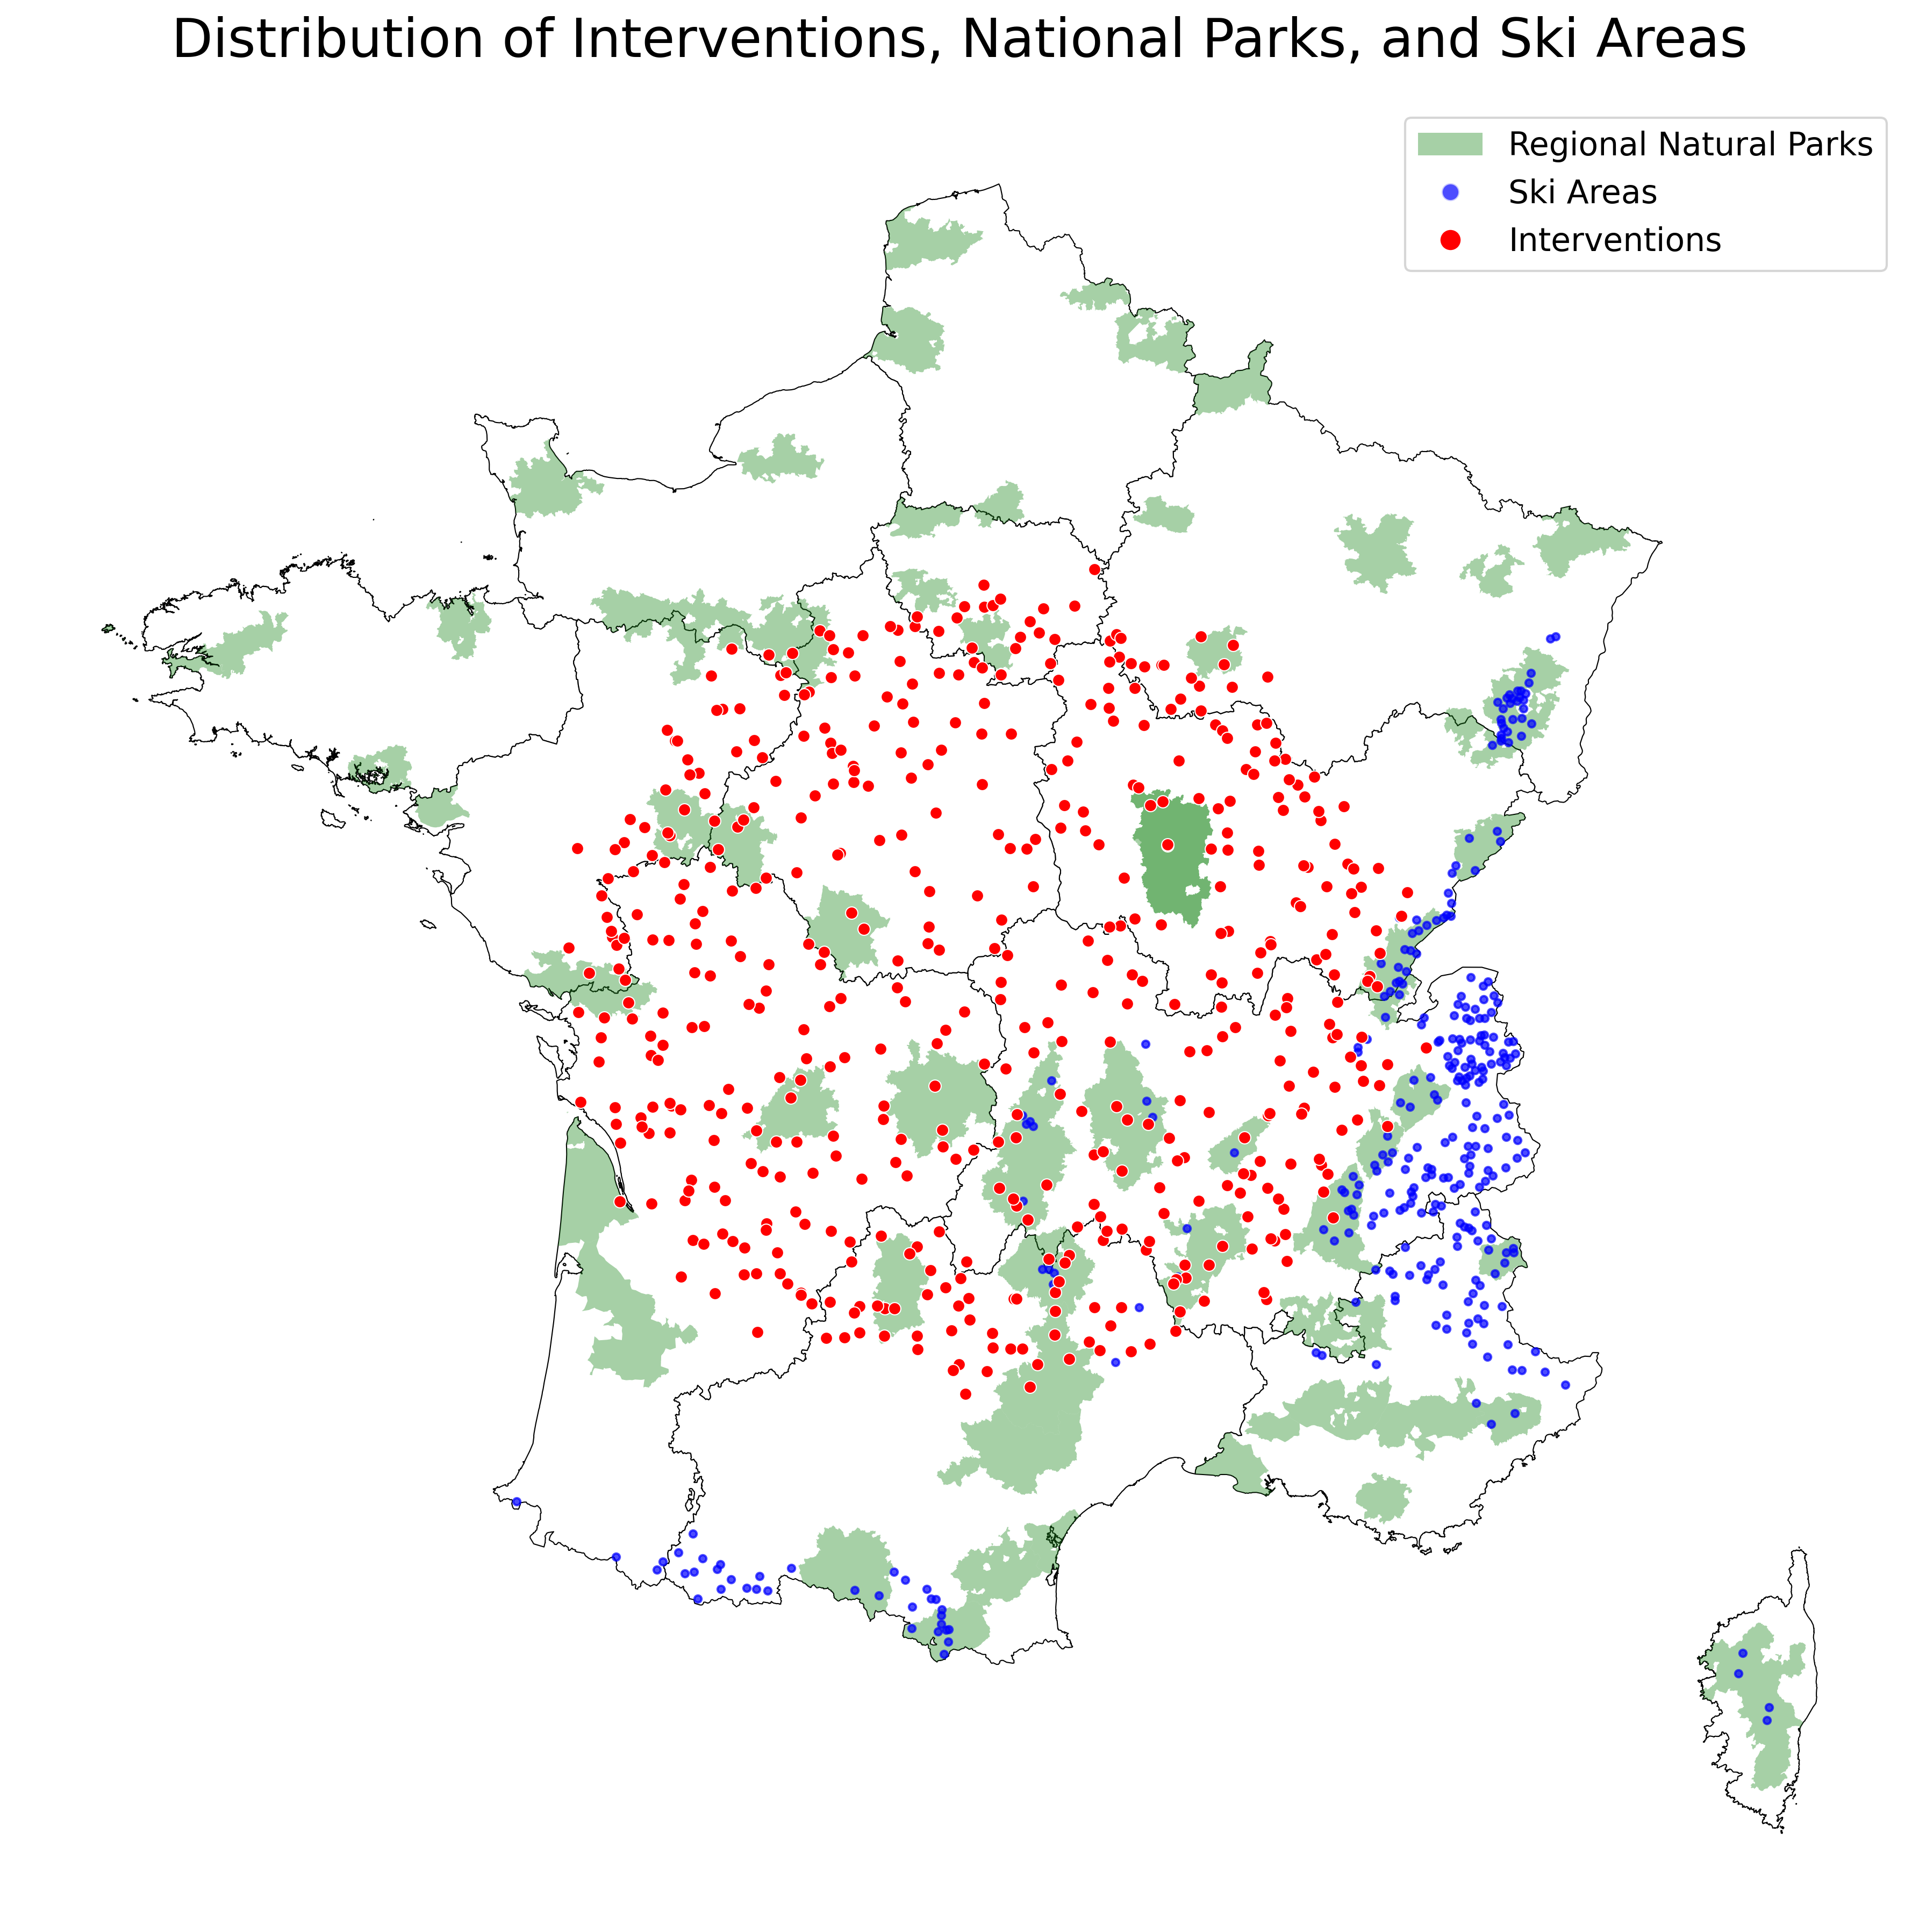
\includegraphics[width=0.8\textwidth]{figures/interventions_map.png}
    \caption{Spatial reconstruction of intervention locations via MDS embedding, overlaid with regional natural parks (green) and ski areas (blue). Each red point represents an intervention projected into the geographical space of France.}
    \label{fig:interventions_map}
\end{figure}

Similarly, the original data encodes the planning horizon as $T=131$ abstract timesteps with seasonal labels (winter, interseason, summer) but no explicit calendar dates. To evaluate criteria that depend on specific periods, such as ski season, summer months, or weekends, a piecewise mapping is constructed. Each seasonal block is assigned to its corresponding calendar months (e.g., winter to January, February, November, and December; summer to May through August). Since each block contains fewer timesteps than calendar days, each timestep is mapped to a contiguous interval of several days, partitioning the block evenly. This alignment enables the identification of weekend overlaps and season-specific windows required by the strategic criteria defined below.

\subsection{Grid Safety and Operational Stability}

The first block of criteria addresses the physical reliability of the grid. Unlike standard mean risk metrics, these indicators focus on tail risks and worst-case scenarios.

\textbf{Reliability Stress ($c_1$):} Optimization algorithms often lower the average risk by allowing short periods of extreme vulnerability. To penalize this, Reliability Stress is defined as the accumulated severity of events exceeding a safety margin. Let $\tau_{90}$ be the 90th percentile of the set $\{R_t : R_t > 0\}$ across the horizon. The integral of the daily risk curve that exceeds this threshold is calculated, favoring schedules that consistently stay within safe operational bounds:
\[
c_1 = \sum_{t=1}^{T} \max(0, R_t - \tau_{90})
\]

\textbf{Max Critical Overlap ($c_2$):} The set $\mathcal{I}_{crit}$ contains the top 10\% of interventions ranked by their mean risk $\bar{r}_i$. This metric records the maximum number of critical tasks active simultaneously at any timestep. Minimizing this overlap reduces the probability of cascading failures caused by simultaneous maintenance on high-voltage lines:
\[
c_2 = \max_{t \in [1, T]} \left| \mathcal{A}_t \cap \mathcal{I}_{crit} \right|
\]

\subsection{Robustness and Resilience}

The second block evaluates the schedule's capacity to absorb unexpected disruptions without becoming infeasible or unsafe.

\textbf{Risk Volatility ($c_3$):} A schedule with gradual risk transitions is inherently more stable against unforeseen events. When the daily risk profile changes smoothly, operational adjustments can be made incrementally, leaving room to accommodate deviations from the plan. Conversely, abrupt transitions leave little margin: any unexpected event (task delay, resource shortage, equipment failure) occurring during a rapid change can push the system into a critical state. Volatility is measured as the total variation of the risk curve:
\[
c_3 = \sum_{t=2}^{T} | R_t - R_{t-1} |
\]

\textbf{Robustness Slack ($c_4$):} This metric identifies the tightest bottleneck. For every resource $r \in \mathcal{R}$ and timestep $t$, the normalized slack between capacity and load is calculated. The metric returns the minimum slack observed across the entire horizon. Unlike the other criteria, this is a maximization objective; a higher value implies that the schedule operates far from saturation points, offering a buffer against unforeseen constraints:
\[
c_4 = \min_{t \in [1,T],\, r \in \mathcal{R}} \left( \frac{C_{r,t}^{max} - L_{r,t}}{C_{r,t}^{max} - C_{r,t}^{min}} \right)
\]

\subsection{Strategic and Socio-Environmental Constraints}

The final block captures ``soft constraints'' related to economic, social, and environmental externalities. These employ the fuzzy-spatial memberships to contextualize the maintenance impact.

\textbf{Ski Season Risk ($c_5$):} Grid failures near mountain resorts during the winter high season result in disproportionate economic and reputational damage. This is quantified by weighting the risk of each active intervention by its fuzzy proximity to known ski stations, summing only during winter months:
\[
c_5 = \sum_{t \in \mathcal{T}_{winter}} \sum_{i \in \mathcal{A}_t} \bar{r}_{i,t} \cdot \mu_{ski}(i)
\]

\textbf{Summer Eco-Stress ($c_6$):} Maintenance in protected nature reserves is restricted during summer to mitigate fire risks and preserve tourism. The daily environmental impact $E_t$ aggregates the park proximity memberships of all active interventions. Let $\tilde{E}$ be the median of $\{E_t\}_{t=1}^{T}$ across the entire horizon. The metric penalizes the integral of this impact that exceeds this baseline during summer, encouraging the shifting of environmentally intrusive tasks to off-peak seasons:
\[
c_6 = \sum_{t \in \mathcal{T}_{summer}} \max(0, E_t - \tilde{E})
\]

\textbf{Social Weekend Risk ($c_7$):} To minimize labor friction and overtime costs, operators aim to avoid starting difficult tasks on weekends. Let $P_{80}$ be the 80th percentile of $\{\bar{r}_i : i \in \mathcal{I}\}$, and let $s_i$ denote the start timestep of intervention $i$. The metric counts heavy interventions starting on weekends:
\[
c_7 = \sum_{i \in \mathcal{I}} \mathbb{I}\bigl(s_i \in \mathcal{T}_{weekend} \land \bar{r}_i > P_{80}\bigr)
\]

\subsection{Alternative Generation}

The choice set comprises schedules generated by three leading algorithms from the ROADEF/EURO 2020 challenge \cite{roadef2020}, selected from among the 13 finalists as the only ones with publicly available compiled code. The first is the winning algorithm by \citet{top1roadef}, a scenario-penalization matheuristic that iteratively solves integer linear programs with dynamically updated objective coefficients (penalties) to effectively approximate and minimize the complex non-linear risk distribution objective. The second is the third-place matheuristic by \citet{Consueloroadef}, which follows a three-phase pipeline: an iterative integer linear programming procedure to generate a pool of initial solutions, a Variable Neighbourhood Descent (VND) for local search, and a Path Relinking procedure for search intensification. The third is the junior-category winner by \citet{top5roadef}, which relies on Mixed-Integer Linear Programming accelerated by an effective greedy initialization.

Each algorithm was executed on instance \texttt{X12}, which was among the most challenging ones due to its size and variability of the best scores provided in the final round of the competition. Five computation time limits (180s, 300s, 500s, 700s, 900s) and three random seeds were used, yielding 45 candidate solutions. After removing 4 infeasible runs from Langiu's algorithm and eliminating 10 duplicates, the final choice set contains $N=31$ distinct alternatives.

\subsection{Matrix Normalization}

The evaluation of these $N$ schedules yields a raw decision matrix $\mathbf{X} \in \mathbb{R}^{N \times 7}$ with multiple different units. To perform a coherent aggregation, max-normalization is applied. All criteria are transformed to a benefit scale where $x_{ij} = 1$ represents the best observed performance:
\[
x_{ij} = \begin{cases}
\dfrac{x^{\mathrm{raw}}_{ij}}{\max_{k} x^{\mathrm{raw}}_{kj}} & \text{if } j=4 \text{ (Robustness Slack)} \\[10pt]
1 - \dfrac{x^{\mathrm{raw}}_{ij} - \min_{k} x^{\mathrm{raw}}_{kj}}{\max_{k} x^{\mathrm{raw}}_{kj}} & \text{otherwise}
\end{cases}
\]
Both cases use max-normalization, mapping values to the interval $[\min/\max, 1]$. For the benefit-type criterion ($c_4$), larger values approach 1. For cost-type criteria, the formula inverts the scale so that the minimum value (best performance) maps exactly to 1, while the maximum maps to $\min/\max$.
